% vim: set tw=78 sts=2 sw=2 ts=8 aw et ai:
\documentclass{workshop}

% Comentează liniile de mai jos în cazul în care nu există cod de inclus.
%\usepackage{code/highlight}
\usepackage{color}        % dacă e folosit highlight
\usepackage{alltt}        % dacă e folosit highlight
\usepackage{verbatim}

\title[Sesssion 10]{Session 10}
\subtitle{Contributing to the Linux Kernel}
\author{Daniel Băluță, Irina Preșa}
\date{July 13, 2012}

\begin{document}

% Arătăm numărul frame-ului
\setbeamertemplate{footline}[frame number]

\frame{\titlepage}

% NB: Secțiunile nu sunt marcate vizual, ci doar apar în cuprins
\section{GIT Versioning Control}

\begin{frame}{GIT Versioning Control}
\begin{itemize}
\item version control software started by Linus Torvalds.
\item high performance for maintaining large projects.
\item<2> "git" $=$ English slang for a stupid or unpleasant person.
\item<2> Torvalds quipped about the name: \emph{"I'm an egotistical bastard, and I
name all my projects after myself. First 'Linux', now 'git'"}.
\end{itemize}
\end{frame}

\begin{frame}{Why Version Control?}
\begin{itemize}
\item restore a previous version.
\item collaborative work.
\item history (comments, changes).
\item branching.
\end{itemize}
\end{frame}

\begin{frame}{Why GIT?}
\begin{itemize}
\item increased performance for large projects.
\item distributed (local vs remote repo).
\item third-party tools/applications integration.
\item track/follow remote repos/branches.
\item extra facilities: stash, index (stage).
\end{itemize}
\end{frame}

\begin{frame}{Repository Architecture}
\begin{figure}
  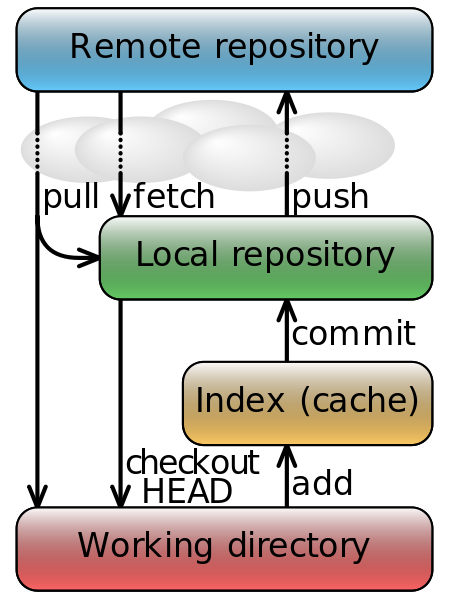
\includegraphics[scale=0.3]{img/flow.png}
\end{figure}
\end{frame}

\begin{frame}{Initial Configurations}
\begin{itemize}
\item git config --global user.name "nume prenume "
\item git config --global user.email "nume@dom.com "
\item git config --global color.ui auto
\item cat /.gitconfig
\end{itemize}
\end{frame}

\begin{frame}{General Flow}
Owner\\
\begin{enumerate}
\item init .
\item create files and directories.
\item add content/modifications to stash: git add.
\item create commit: git commit -m "Message".
\item go back to step 2.
\end{enumerate}
Contribuitor\\
\begin{enumerate}
\item clone repo: git clone URL.
\item create files and directories.
\item add content/modifications to stash: git add.
\item create commit: git commit -m "Message".
\item update local repo: git pull --rebase
\item send modifications: git push origin master
\item go back to step 2.
\end{enumerate}
\end{frame}

\begin{frame}{General Flow}
Owner\\
\begin{enumerate}
\item init .
\item create files and directories.
\item add content/modifications to stash: git add.
\item create commit: git commit -m "Message".
\item go back to step 2.
\end{enumerate}
"Not-trusted" comitter\\
\begin{enumerate}
\item fork repo: git fork URL.
\item create files and directories.
\item add content/modifications to stash: git add.
\item create commit: git commit -m "Message".
\item send modifications: git push origin master
\item go back to step 2.
\item after finishing work:
\begin{itemize}
\item create and send patch OR
\item send pull request
\end{itemize}
\end{enumerate}
\end{frame}

\begin{frame}{Repo Visualization}
\begin{itemize}
\item git diff
\item git status, log
\item git show <rev>
\item git blame <file>
\item gitk, gitg, giggle, tig
\end{itemize}
\end{frame}

\begin{frame}{Solving Conflicts}
\begin{itemize}
\item manual merge or use a special tool
\item git stash
\item git bisect (binary search)
\end{itemize}
\end{frame}

\begin{frame}[fragile]{Solving Conflicts}
\begin{verbatim}
git stash
git pull
git stash pop
//solve conflicts
//commit
\end{verbatim}
\begin{verbatim}
$ git bisect start
$ git bisect bad
$ git bisect good v1.0
Bisecting: 6 revisions left to test after this
[ecb6e1b] error handling on repo
git bisect good/bad
\end{verbatim}
\end{frame}

\begin{frame}{Branching}
\begin{itemize}
\item collaborative editing.
\item faster development.
\item different development branches.
\begin{itemize}
\item new release.
\item experimental feature.
\item new module
\end{itemize}
\end{itemize}
\end{frame}

\begin{frame}{Patching Solutions}
\begin{itemize}
\item git format-patch
\item git send-mail
\item git diff
\end{itemize}
\end{frame}

\begin{frame}{Extra: Post-Receive Hooks}
\begin{itemize}
\item .git/hooks in repo.
\item publish results.
\item create archives.
\item send e-mails.
\end{itemize}
\end{frame}

\section{Linux Kernel development model}

\begin{frame}{Overview}
\begin{figure}
  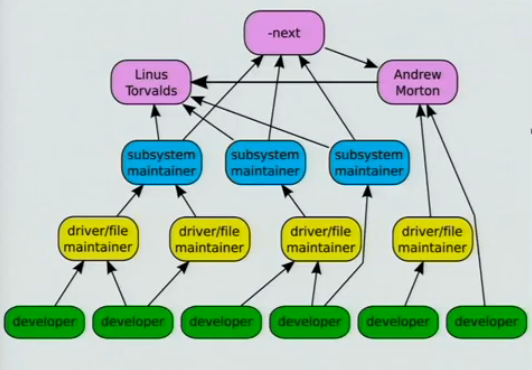
\includegraphics[scale=0.6]{img/trees.png}
\end{figure}

\end{frame}

\begin{frame}{Just a bit of taste}
\begin{itemize}
\item curent versioning scheme: 3.x.y
\begin{itemize}
\item 3.x-rcN, release candidate (each week)
\item 3.x, major release (around 2 months)
\item 3.x.y, minor release (whenever is needed)
\end{itemize}
\item previous versioning scheme: 2.6.x.y
\begin{itemize}
\item 20 years of Linux
\item 2.6.39 switched to 3.0
\end{itemize}
\item case study - 3.4.0 release
\begin{itemize}
\item 2833 developers
\item 373 companies
\item 7.21 changes per hour
\end{itemize}
\end{itemize}
\end{frame}

\begin{frame}{Life of a patch}
\begin{itemize}
\item modify code, and create patch
\item check_maintainer.pl
\item checkpatch.pl
\item send patch to correct recipients
\item wait for feedback
\end{itemize}
\end{frame}



\section{Keywords}

\begin{frame}{Keywords}
     \begin{itemize}
	\item git
      \end{itemize}
\end{frame}

\section{Resources}
\begin{frame}{Resources}
  \begin{itemize}
  \item \href{http://cscope.sourceforge.net/cscope_vim_tutorial.html}{Using Cscope with vim}
  \end{itemize}
\end{frame}

\section{Questions}

\end{document}
